\documentclass{standalone}
\usepackage{pgfplots}
\pgfplotsset{compat=1.18}

\begin{document}

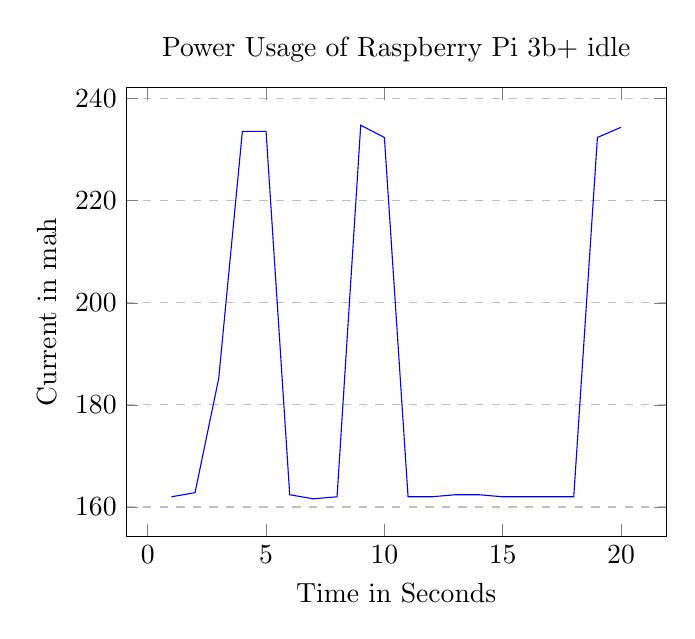
\begin{tikzpicture}
    \begin{axis}[
    title={Power Usage of Raspberry Pi 3b+ idle},
    xlabel={Time in Seconds},
    ylabel={Current in mah},
    %ytick=data,
    %xtick=data,
    ymajorgrids=true,
    legend pos=outer north east,
    grid style=dashed,
    ]
    \addplot[
        color=blue,
    ]
    coordinates {
        (1,162.00)
        (2,162.80)
        (3,185.20)
        (4,233.60)
        (5,233.60)
        (6,162.40)
        (7,161.60)
        (8,162.00)
        (9,234.80)
        (10,232.40)
        (11,162.00)
        (12,162.00)
        (13,162.40)
        (14,162.40)
        (15,162.00)
        (16,162.00)
        (17,162.00)
        (18,162.00)
        (19,232.40)
        (20,234.40)
    };
    \end{axis}
\end{tikzpicture}
\hspace{.5cm}

\end{document}
